%%=============================================================================
%% Prijs vergelijking
%%=============================================================================
\chapter{\IfLanguageName{dutch}{Prijs vergelijking}{Price comparison}}

Met dank aan Robonext\footnote{https://robonext.eu/} voor het voorzien van deze afbeeldingen.

Niet elke provider heeft tijdig gereageerd op de mail met vragen rond de prijs van hun \acrshort{rpa} oplossing.

\section{Marktonderzoek}
De \acrshort{rpa} markt is verdeeld in 4 delen. De 'Big 3', UiPath, Automation Anywhere en BluePrism, nemen ongeveer 70\% van de hele markt op, de overige 30\% wordt opgesplitst onder de rest van de kleinere providers. Hierbij kan een ruwe benadering gevonden worden waarbij UiPath ongeveer 35\% van de markt in zijn bezit heeft, Automation Anywhere dan weer 25\% en tot slot Blueprism die ongeveer 10\% in zijn bezit heeft. \autocite{marktRPA}

Ook kan hierbij de assumptie gemaakt worden dat de hoop van kleine spelers minder en minder relevant worden en dat het uiteindelijk op een competitieve race tussen de 'Big 3' zal uitdraaien. \autocite{marktRPA}

\subsection{'The Big Three'}
Uit de verschillende foto's kan nog maar eens besloten worden dat UiPath het meeste marktaandeel heeft van alle providers en dat de markt gedomineerd wordt door de grote drie spelers binnen de markt. 
\begin{figure}[h!]
	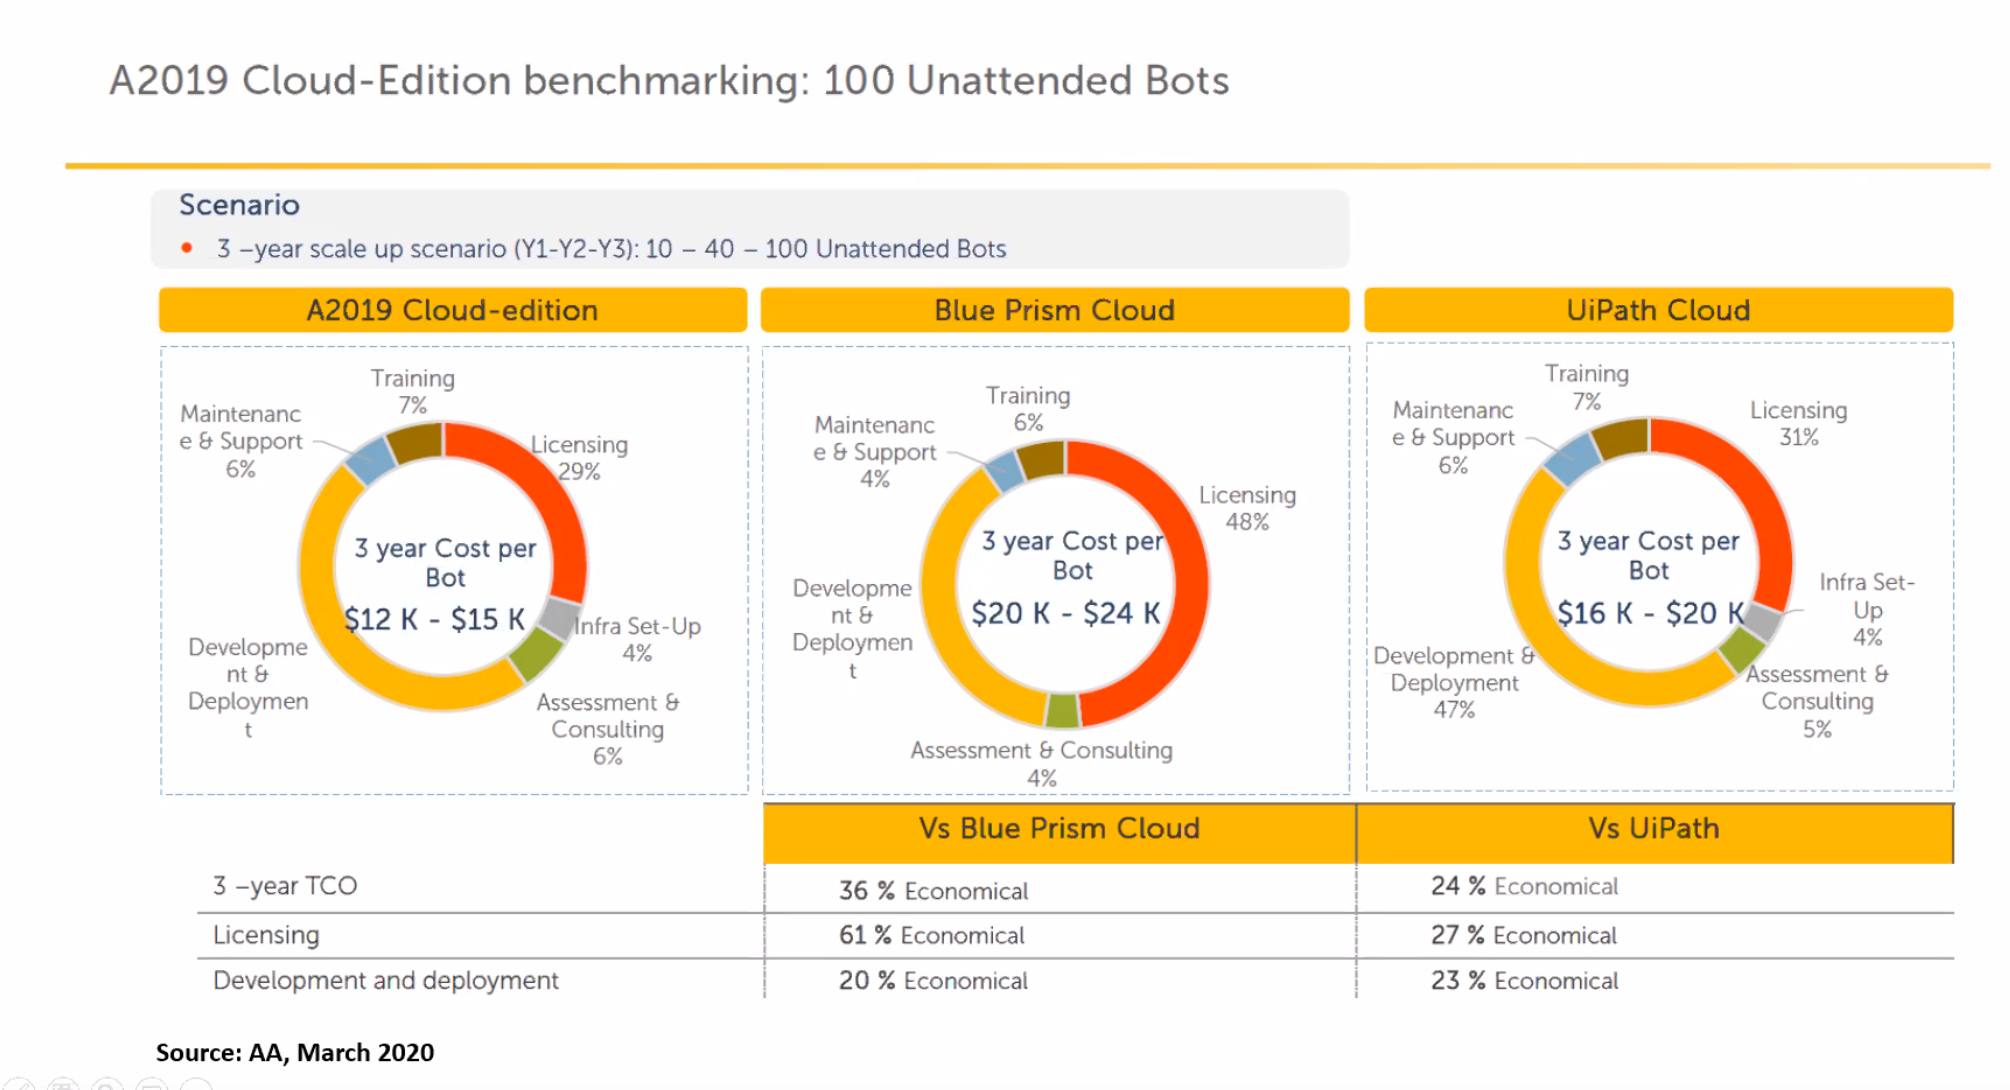
\includegraphics[width=\linewidth]{pricing/price_comparison_1.png}
	\caption[Cloud editie benchmarks]{Het verschil in prijs voor een cloud oplossing bij de grote 3 RPA providers.}
	\label{fig:price_1}
\end{figure}
\begin{figure}[h!]
	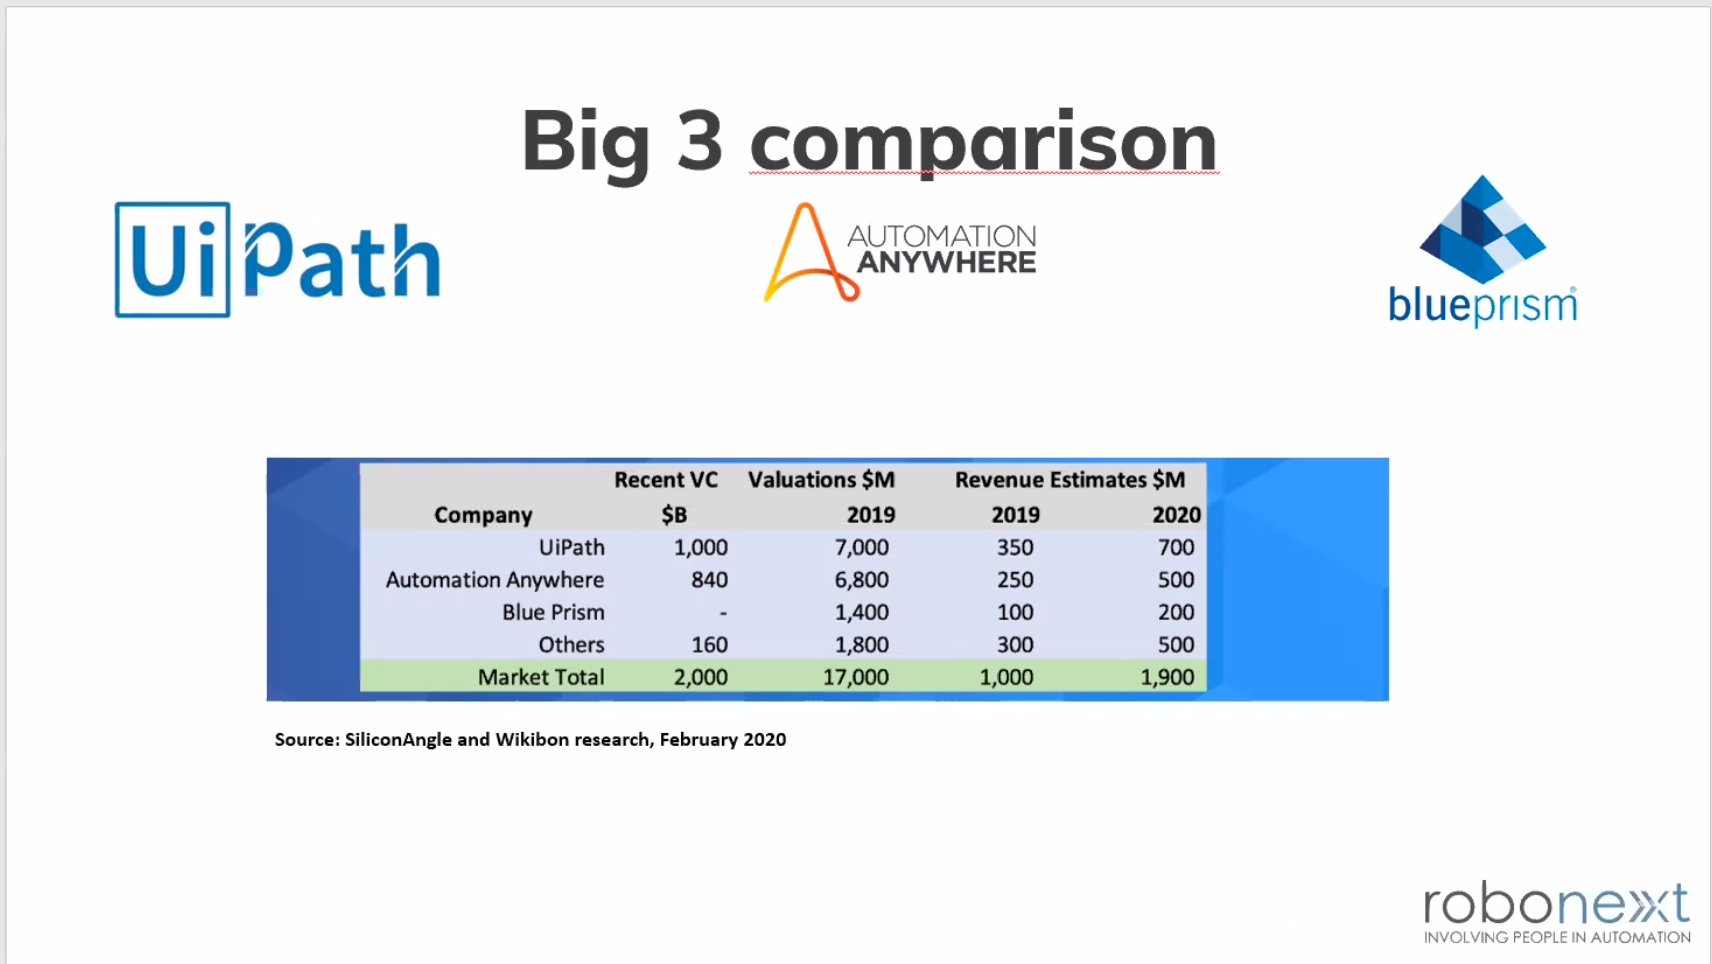
\includegraphics[width=\linewidth]{pricing/price_comparison_2.png}
	\caption[Grote 3 Revenue Streams]{Schatting naar marktwaarden en marktaandeel van de grote 3 ten opzichte van de rest.}
	\label{fig:price_2}
\end{figure}
\begin{figure}[h!]
	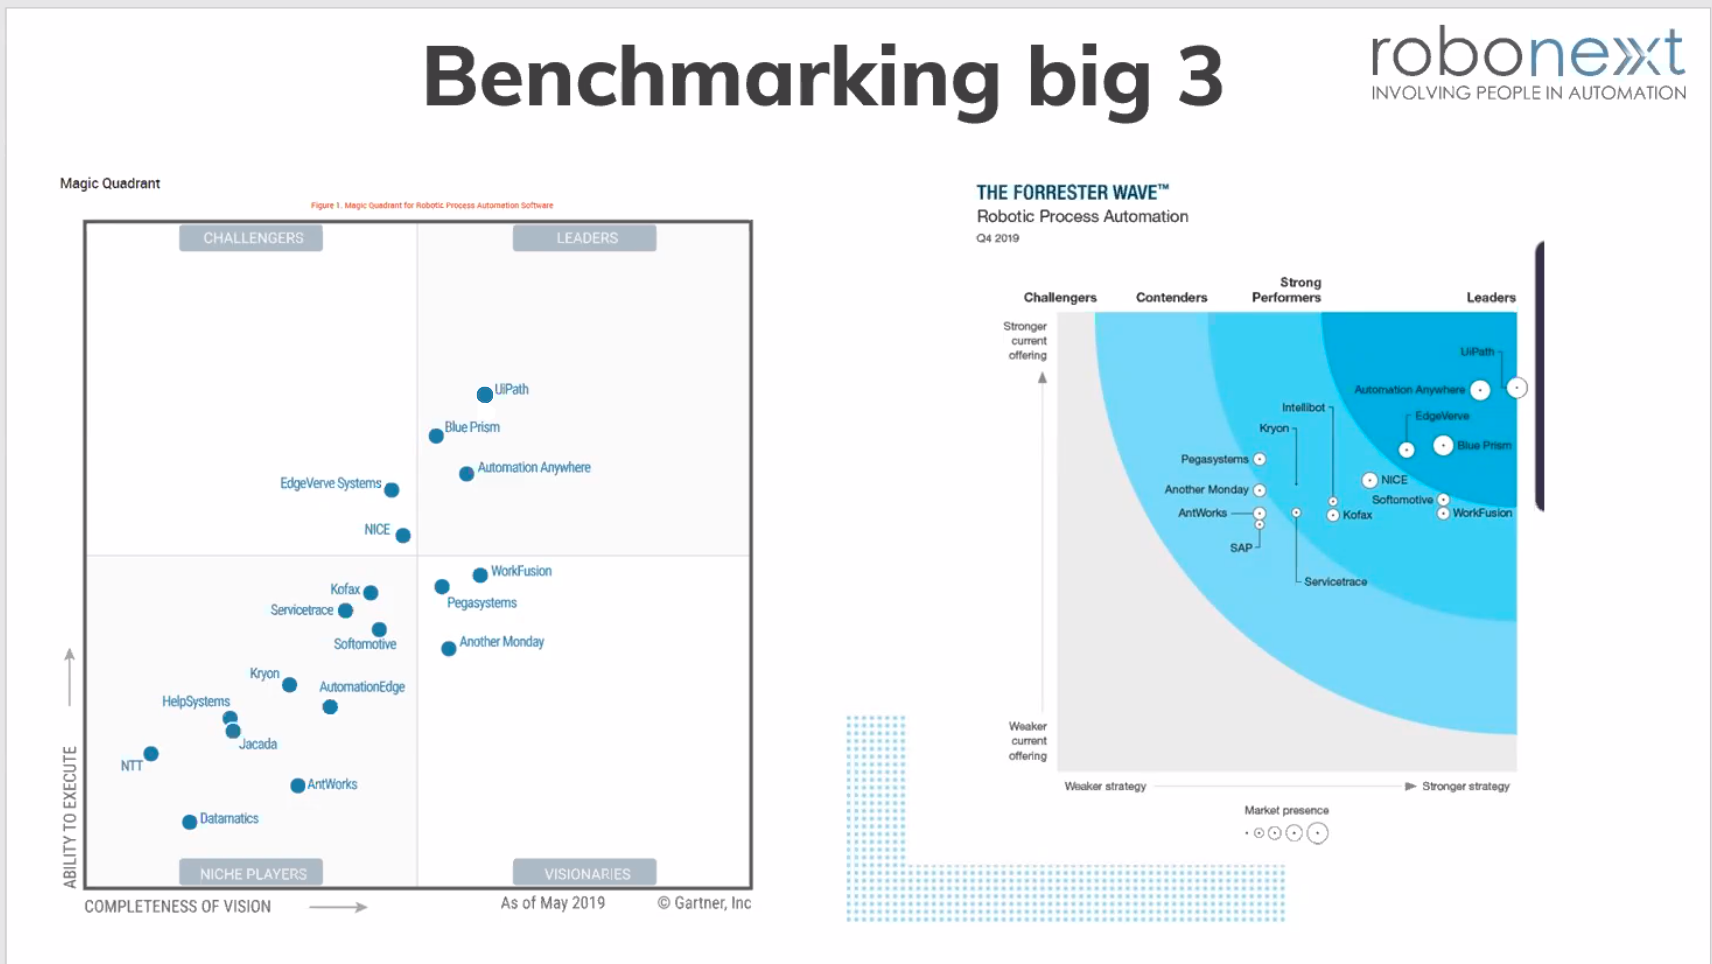
\includegraphics[width=\linewidth]{pricing/price_comparison_3.png}
	\caption[Benchmarkings]{De marktleiders en de opkomende spelers.}
	\label{fig:price_3}
\end{figure}

\subsection{Microsoft Flow}
Als niet traditionele \acrshort{rpa} provider wil Microsoft zich ook competitief op de markt zetten met Flow die een sterken samenhang kent met Power Apps en Azure. Hierbij wordt gewerkt met licenties en subscripties.
\begin{figure}[h!]
	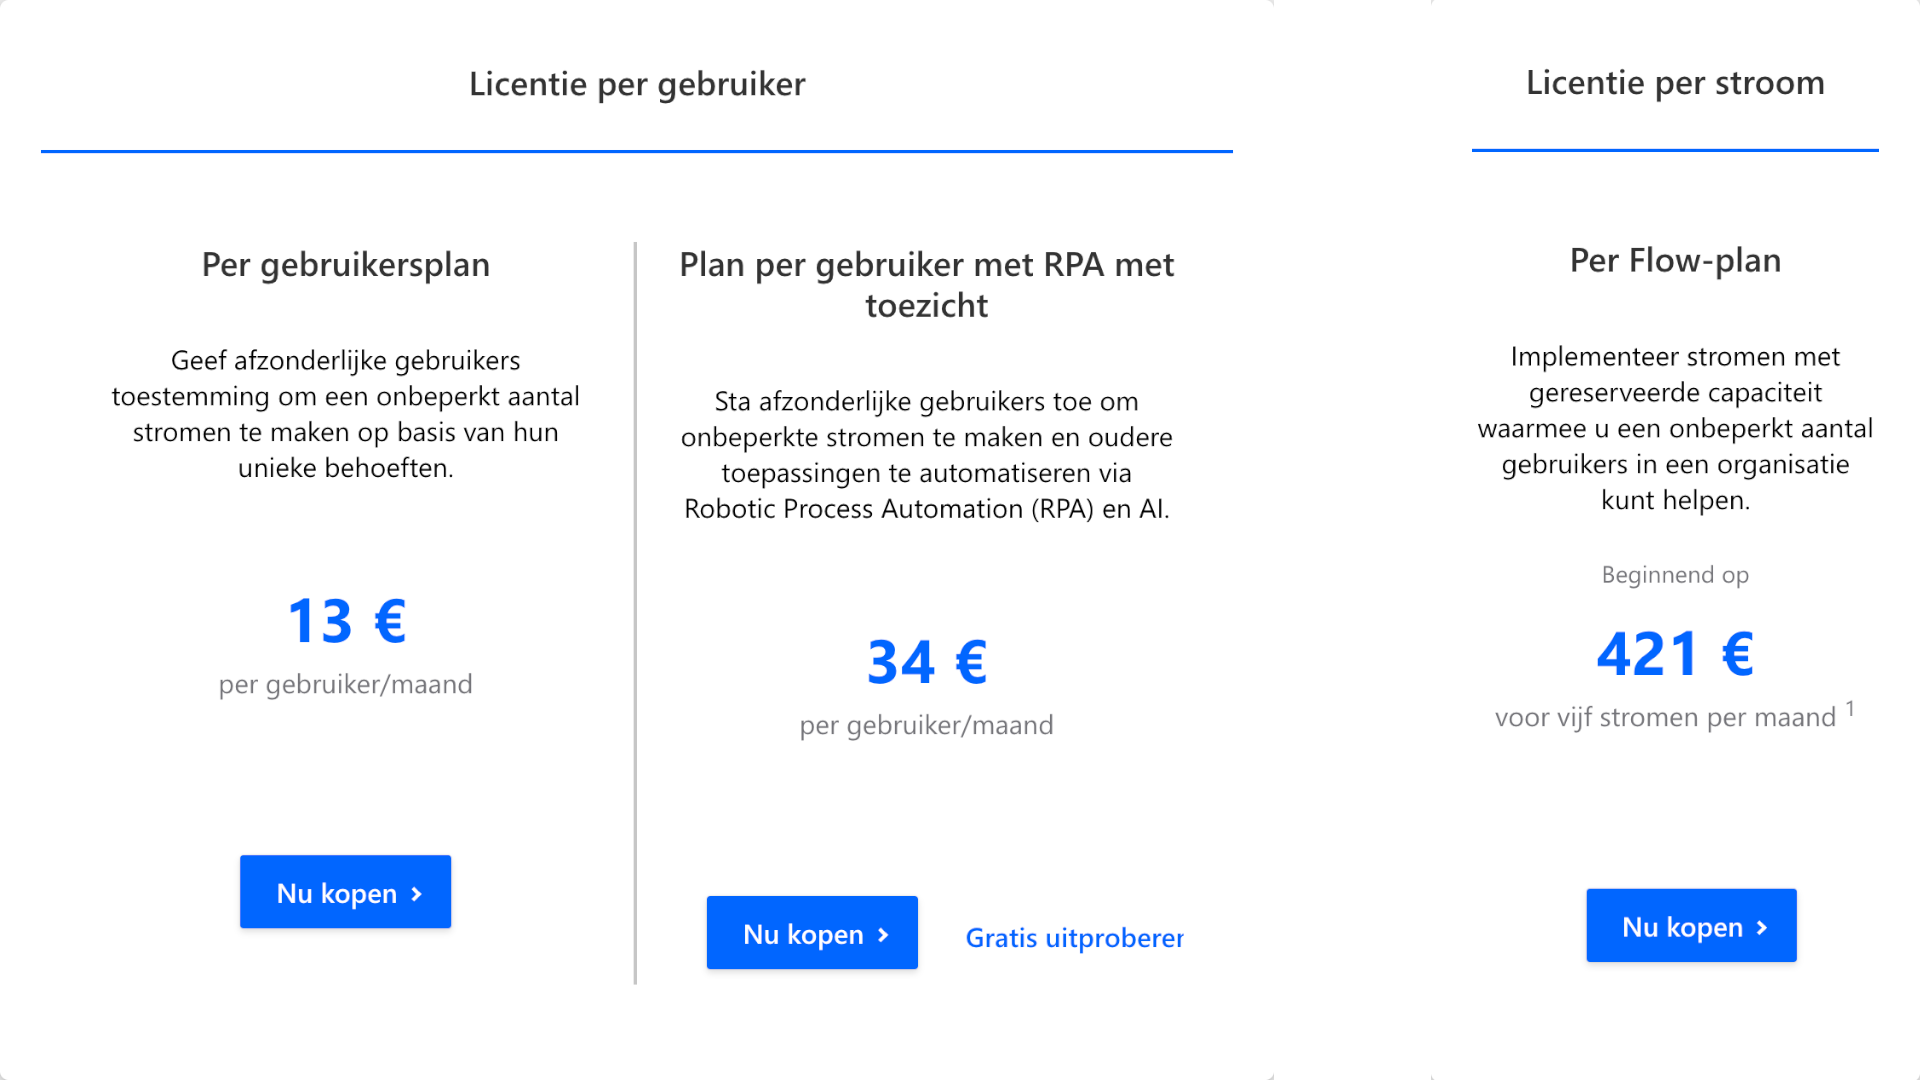
\includegraphics[width=\linewidth]{pricing/price_mf_1.png}
	\caption[Microsoft Flow licenties]{Prijs van de verschillende licenties van Microsoft Flow.}
	\label{fig:price_mf_1}
\end{figure}

\begin{figure}[h!]
	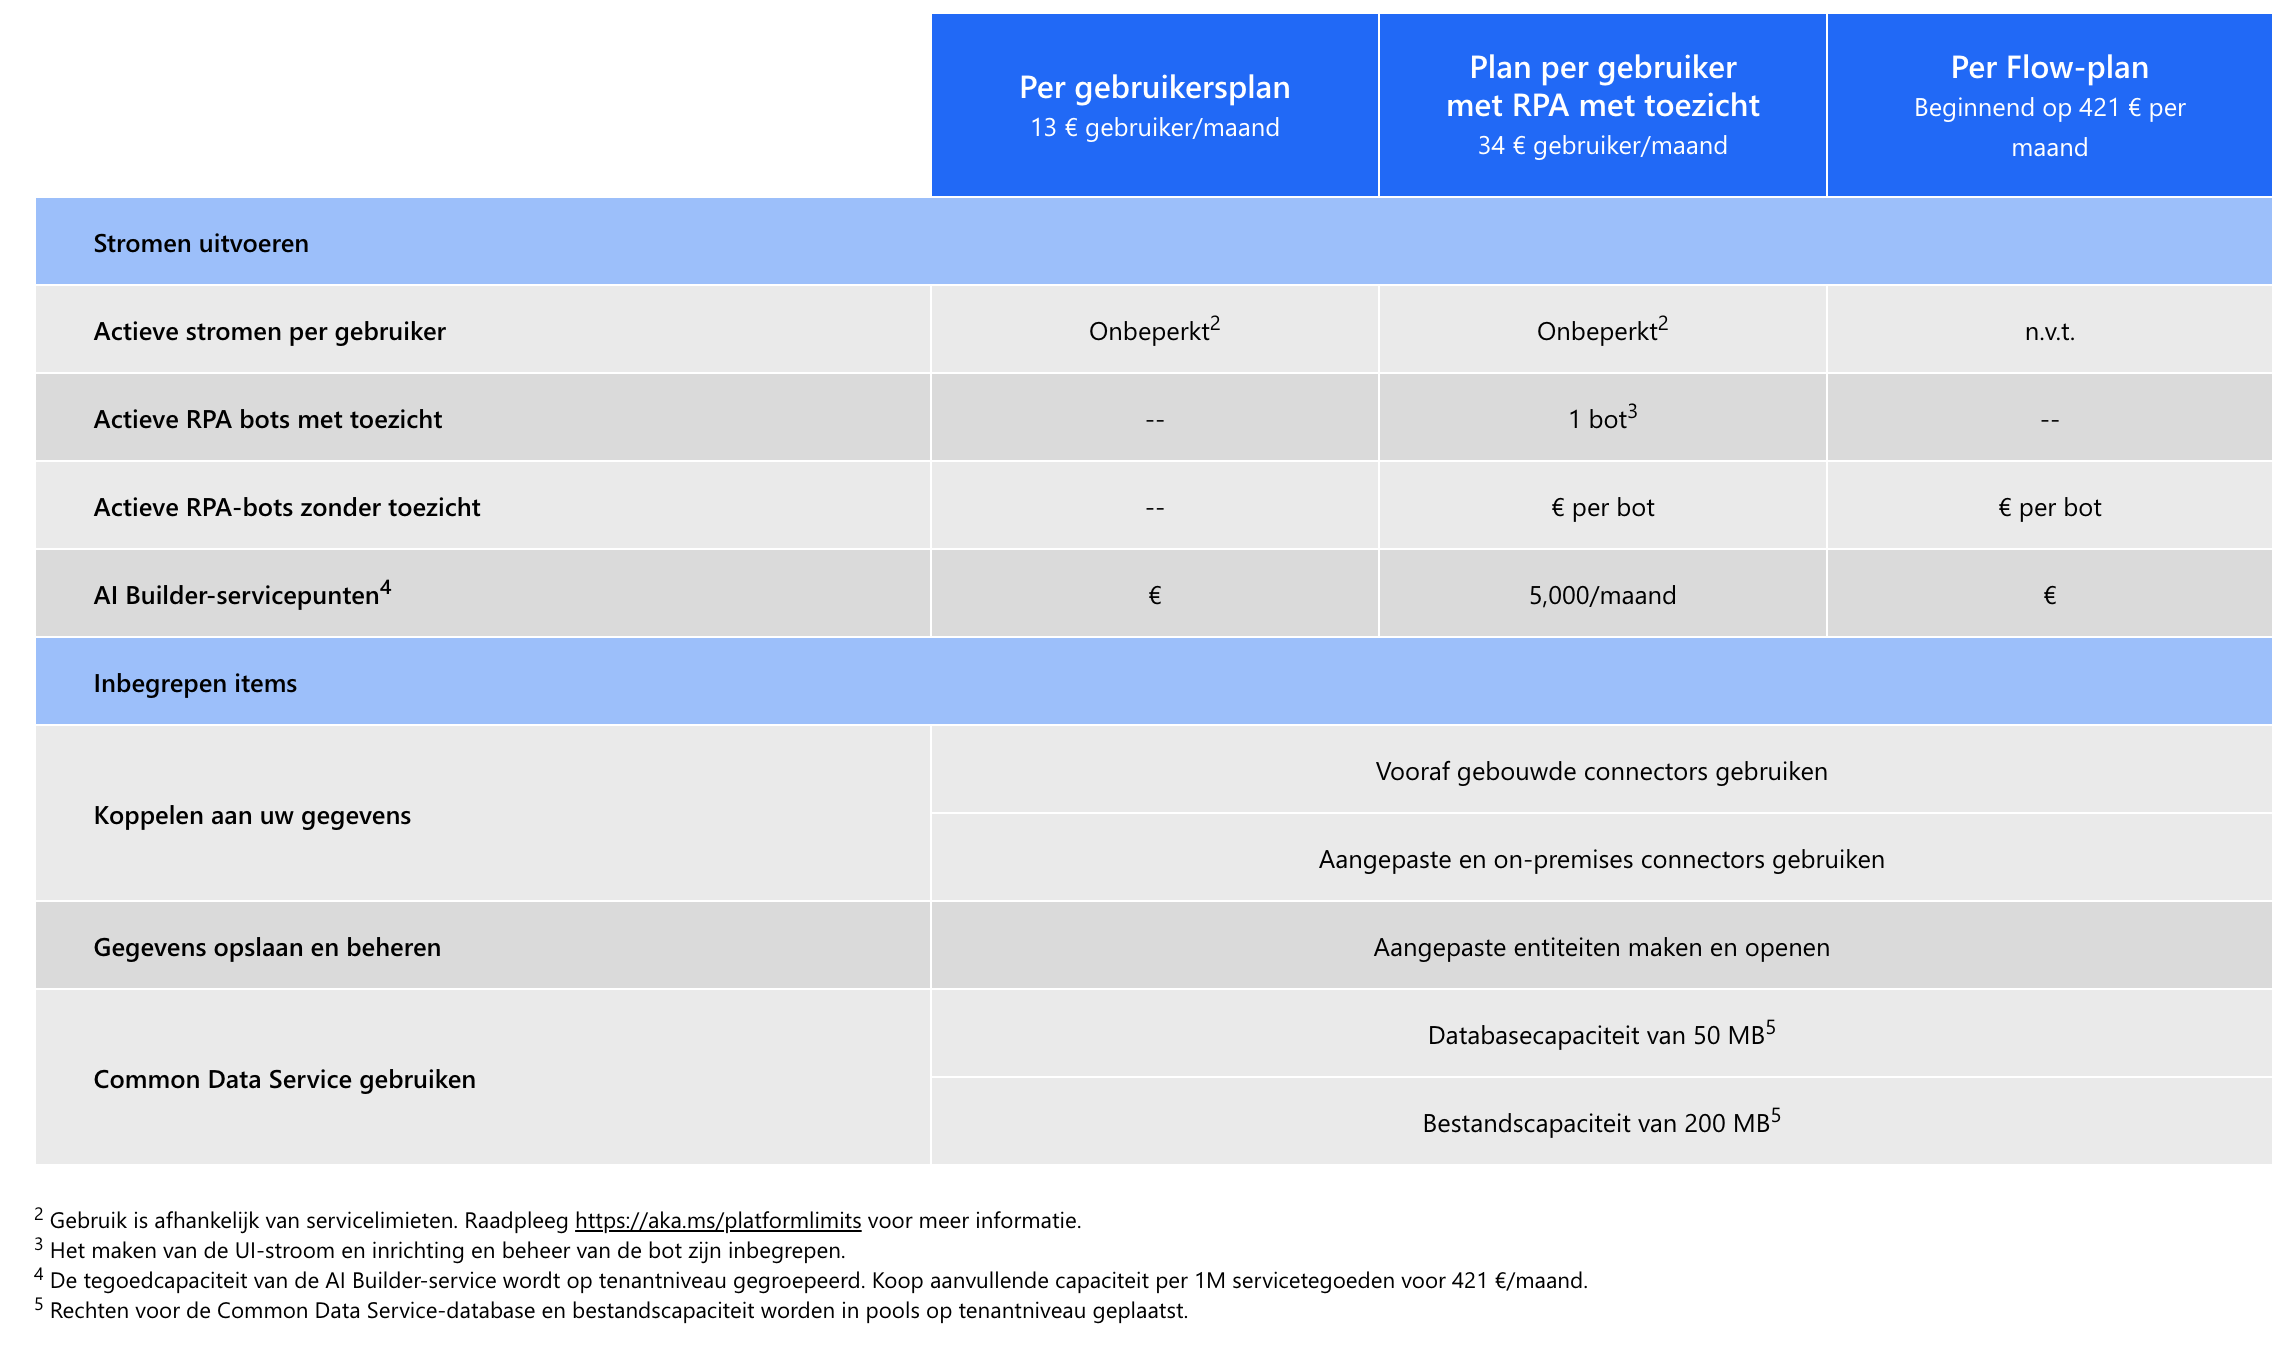
\includegraphics[width=\linewidth]{pricing/price_mf_2.png}
	\caption[Microsoft Flow gebruikersplan]{Prijs voor de verschillende gebruikersplannen bij Microsoft Flow.}
	\label{fig:price_mf_2}
\end{figure}

\begin{figure}[h!]
	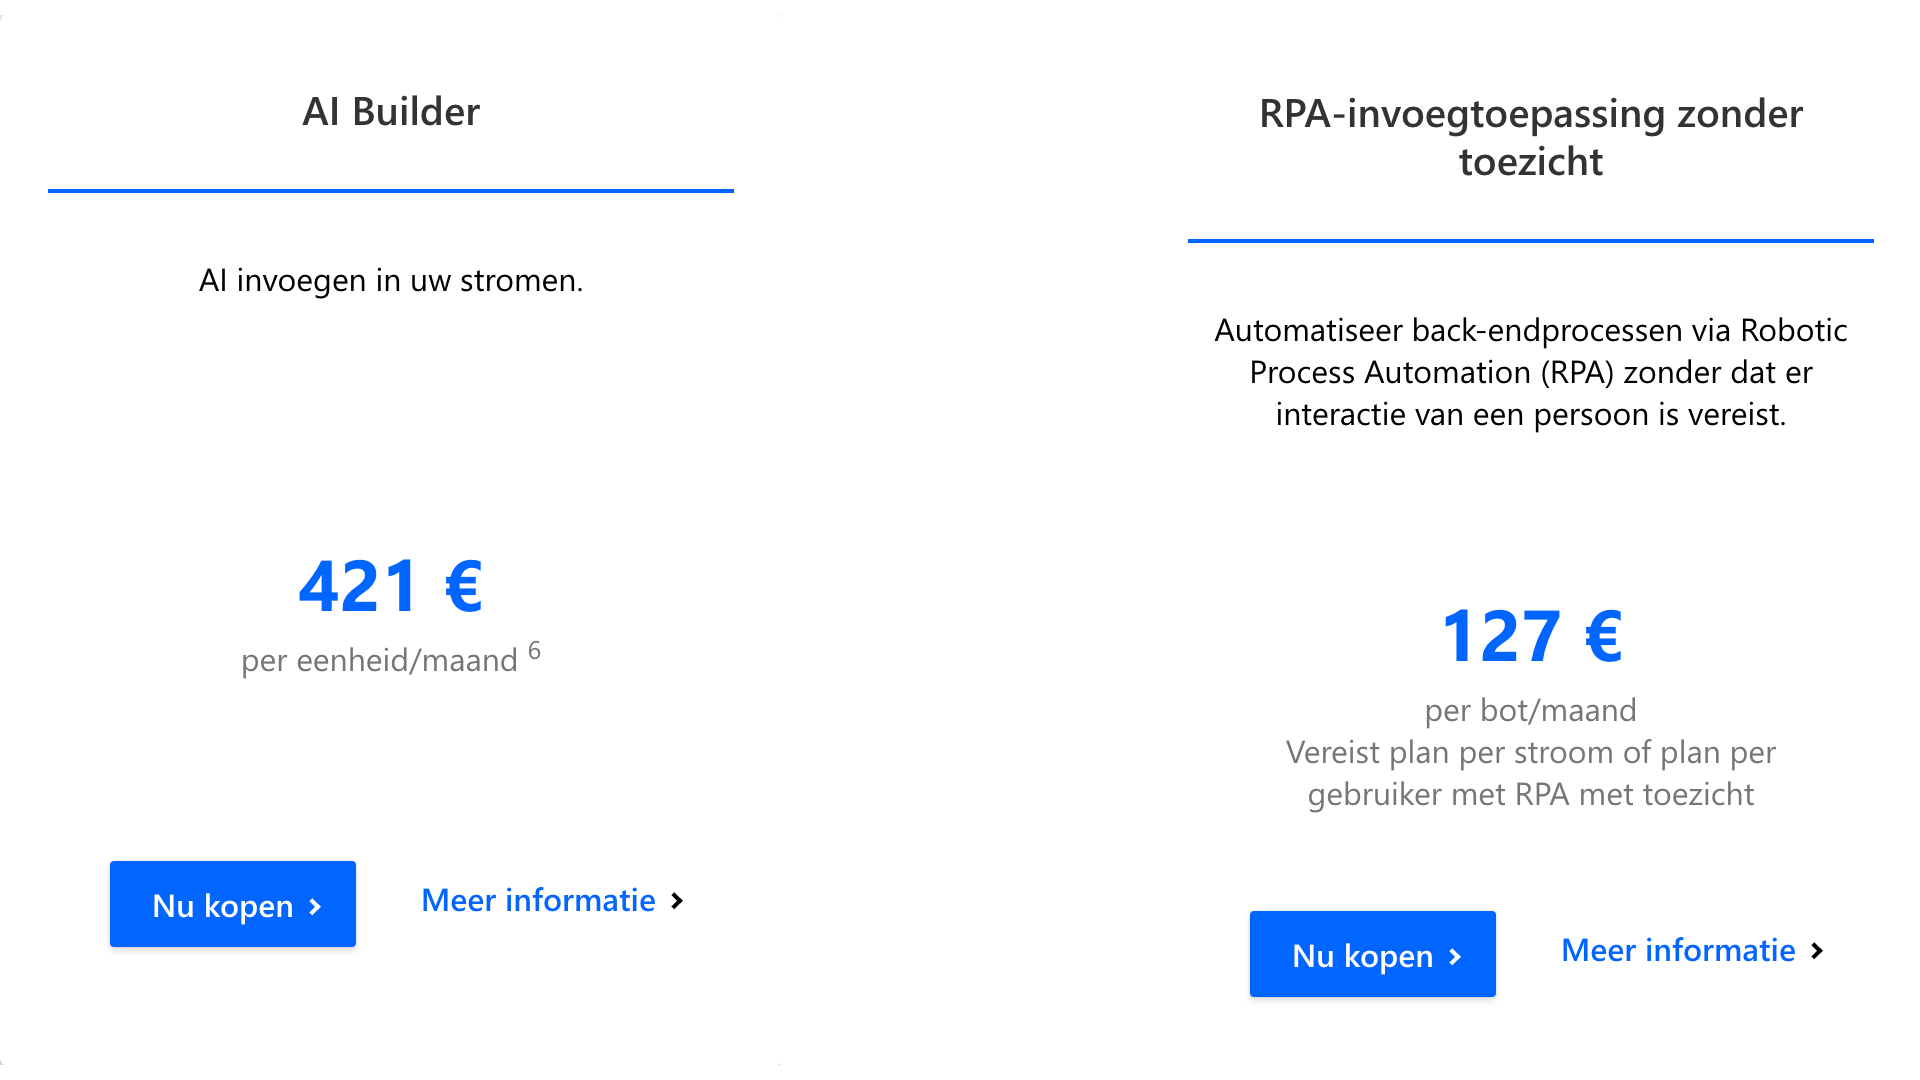
\includegraphics[width=\linewidth]{pricing/price_mf_3.png}
	\caption[Microsoft Flow extra services]{Prijs voor extra services bij Microsoft Flow.}
	\label{fig:price_mf_3}
\end{figure}